\section{Analysis of Applications}
\label{sec:classification}





\subsection{Traffic Classification Methodology}

Why do we need to classify traffic?
Why is it traffic classification important?
How is it useful?
How have previous work used traffic classification?

Use well known port numbers to broadly categorize tcp and udp traffic. 
TCP traffic is classified as either HTTP, SSL, or other while UDP is classified as either DNS or other. 
SSL: 443/tcp, 563/tcp, 585/tcp, 614/tcp, 636/tcp, 989/tcp, 990/tcp, 992/tcp, 993/tcp, 995/tcp, 5223/tcp.
HTTP:  80/tcp, 81/tcp, 631/tcp, 1080/tcp, 3138/tcp, 8000/tcp, 8080/tcp, 8888/tcp.
Traffic such as ICMP which is neither TCP or UDP is classified as other. 
In \fref{tab:summaryIOSAndroidTraffic} we observe that based on this simple classification we observe that more than 90\% of the traffic is either HTTP or SSL.
We observe that the traffic share of SSL over cellular is more than twice the traffic share observed over \wifi  

\subsubsection{Classification of HTTP Traffic}

Why IP and DNS is not sufficient?
User-Agent field 
Limitation of User-Agent field 


\subsubsection{Classification of SSL Traffic}

\subsection{Traffic Characteristics of iOS and Android Applications}


\subsection{Controlled Experiments on }



\begin{enumerate}
\item Traffic classification: Is it possible to identify the source of the traffic by just looking at the traffic? What heuristics can be used? What fraction of the traffic can be classified to specific webservices?
\item Traffic characteristics: What are the network traffic characteristics of popular webservices/apps? Impact of the access technology and operating system on the webservices? 
\item Information exchange: How are CDNs and other servers used? What fraction of traffic is due to ads and analytics and other trackers? How frequently is PII leaked and to which hosts?
\end{enumerate}

\begin{table}
\begin{center}
\begin{tabular}{|p{0.15\columnwidth}|p{0.12\columnwidth}|r|r|r|r|}
\hline
\multirow{2}{*}{\bf Protocol} & \multirow{2}{*}{\bf Service} & \multicolumn{2}{|c|}{\bf Android} & \multicolumn{2}{|c|}{\bf iOS} \tabularnewline
\cline{3-6}
           &           &  \textbf{Cell.}  &  \textbf{\wifi}  &  \textbf{Cell.}  &  \textbf{\wifi}  \tabularnewline
\hline
\multirow{3}{*}{TCP}
       &  HTTP  & 35.386 & 68.686 & 52.109 & 75.506 \tabularnewline
\cline{2-6}
       &  SSL   & 61.134 & 24.366 & 46.765 & 15.777 \tabularnewline
\cline{2-6}
       &  other & 2.346  & 6.290  & 0.256  & 1.818 \tabularnewline
\hline
\multirow{2}{*}{UDP}
       &  DNS   & 0.681  & 0.496  & 0.545  & 0.305  \tabularnewline
\cline{2-6}
       &  other & 0.315  & 0.096  & 0.283  & 6.580  \tabularnewline
\hline
 Other &  -     & 0.134  & 0.062 & 0.039  & 0.011  \tabularnewline
\hline
\multicolumn{2}{|c|}{\emph{total}} & 100.00 & 100.00 & 100.00 & 100.00 \tabularnewline
\hline
\end{tabular}
\end{center}
\caption{Traffic volume (in percentage) of popular protocols on Android and iOS devices over cellular and \wifi.
\tbd{Verify total 100 for final results}
 \emph{Traffic share of SSL over cellular networks is more than twice the traffic share of SSL over \wifi.}} 
\label{tab:summaryIOSAndroidTraffic}
\end{table}

Use well known port numbers to broadly categorize tcp and udp traffic. 
TCP traffic is classified as either HTTP, SSL, or other while UDP is classified as either DNS or other. 
SSL: 443/tcp, 563/tcp, 585/tcp, 614/tcp, 636/tcp, 989/tcp, 990/tcp, 992/tcp, 993/tcp, 995/tcp, 5223/tcp.
HTTP:  80/tcp, 81/tcp, 631/tcp, 1080/tcp, 3138/tcp, 8000/tcp, 8080/tcp, 8888/tcp.
Traffic such as ICMP which is neither TCP or UDP is classified as other. 
In \fref{tab:summaryIOSAndroidTraffic} we observe that based on this simple classification we observe that more than 90\% of the traffic is either HTTP or SSL.
We observe that the traffic share of SSL over cellular is more than twice the traffic share observed over \wifi  

\subsection{Classification of HTTP Traffic}

A mobile application can append information about the application, carrier, and other information related to the device in the User-Agent field. 
Webservices use this information to segregate traffic from the mobile devices and carriers and to offer custom services.  
Recent studies on mobile traffic classification have used the User-Agent field to classify mobile HTTP traffic~\cite{qian:webcache, maier:mobtraffic, xu:appusage}.
We now provide a comparison on the usefulness of the User-Agent field when classifying mobile traffic and discuss the issues with Android devices and media traffic. 

\begin{figure}
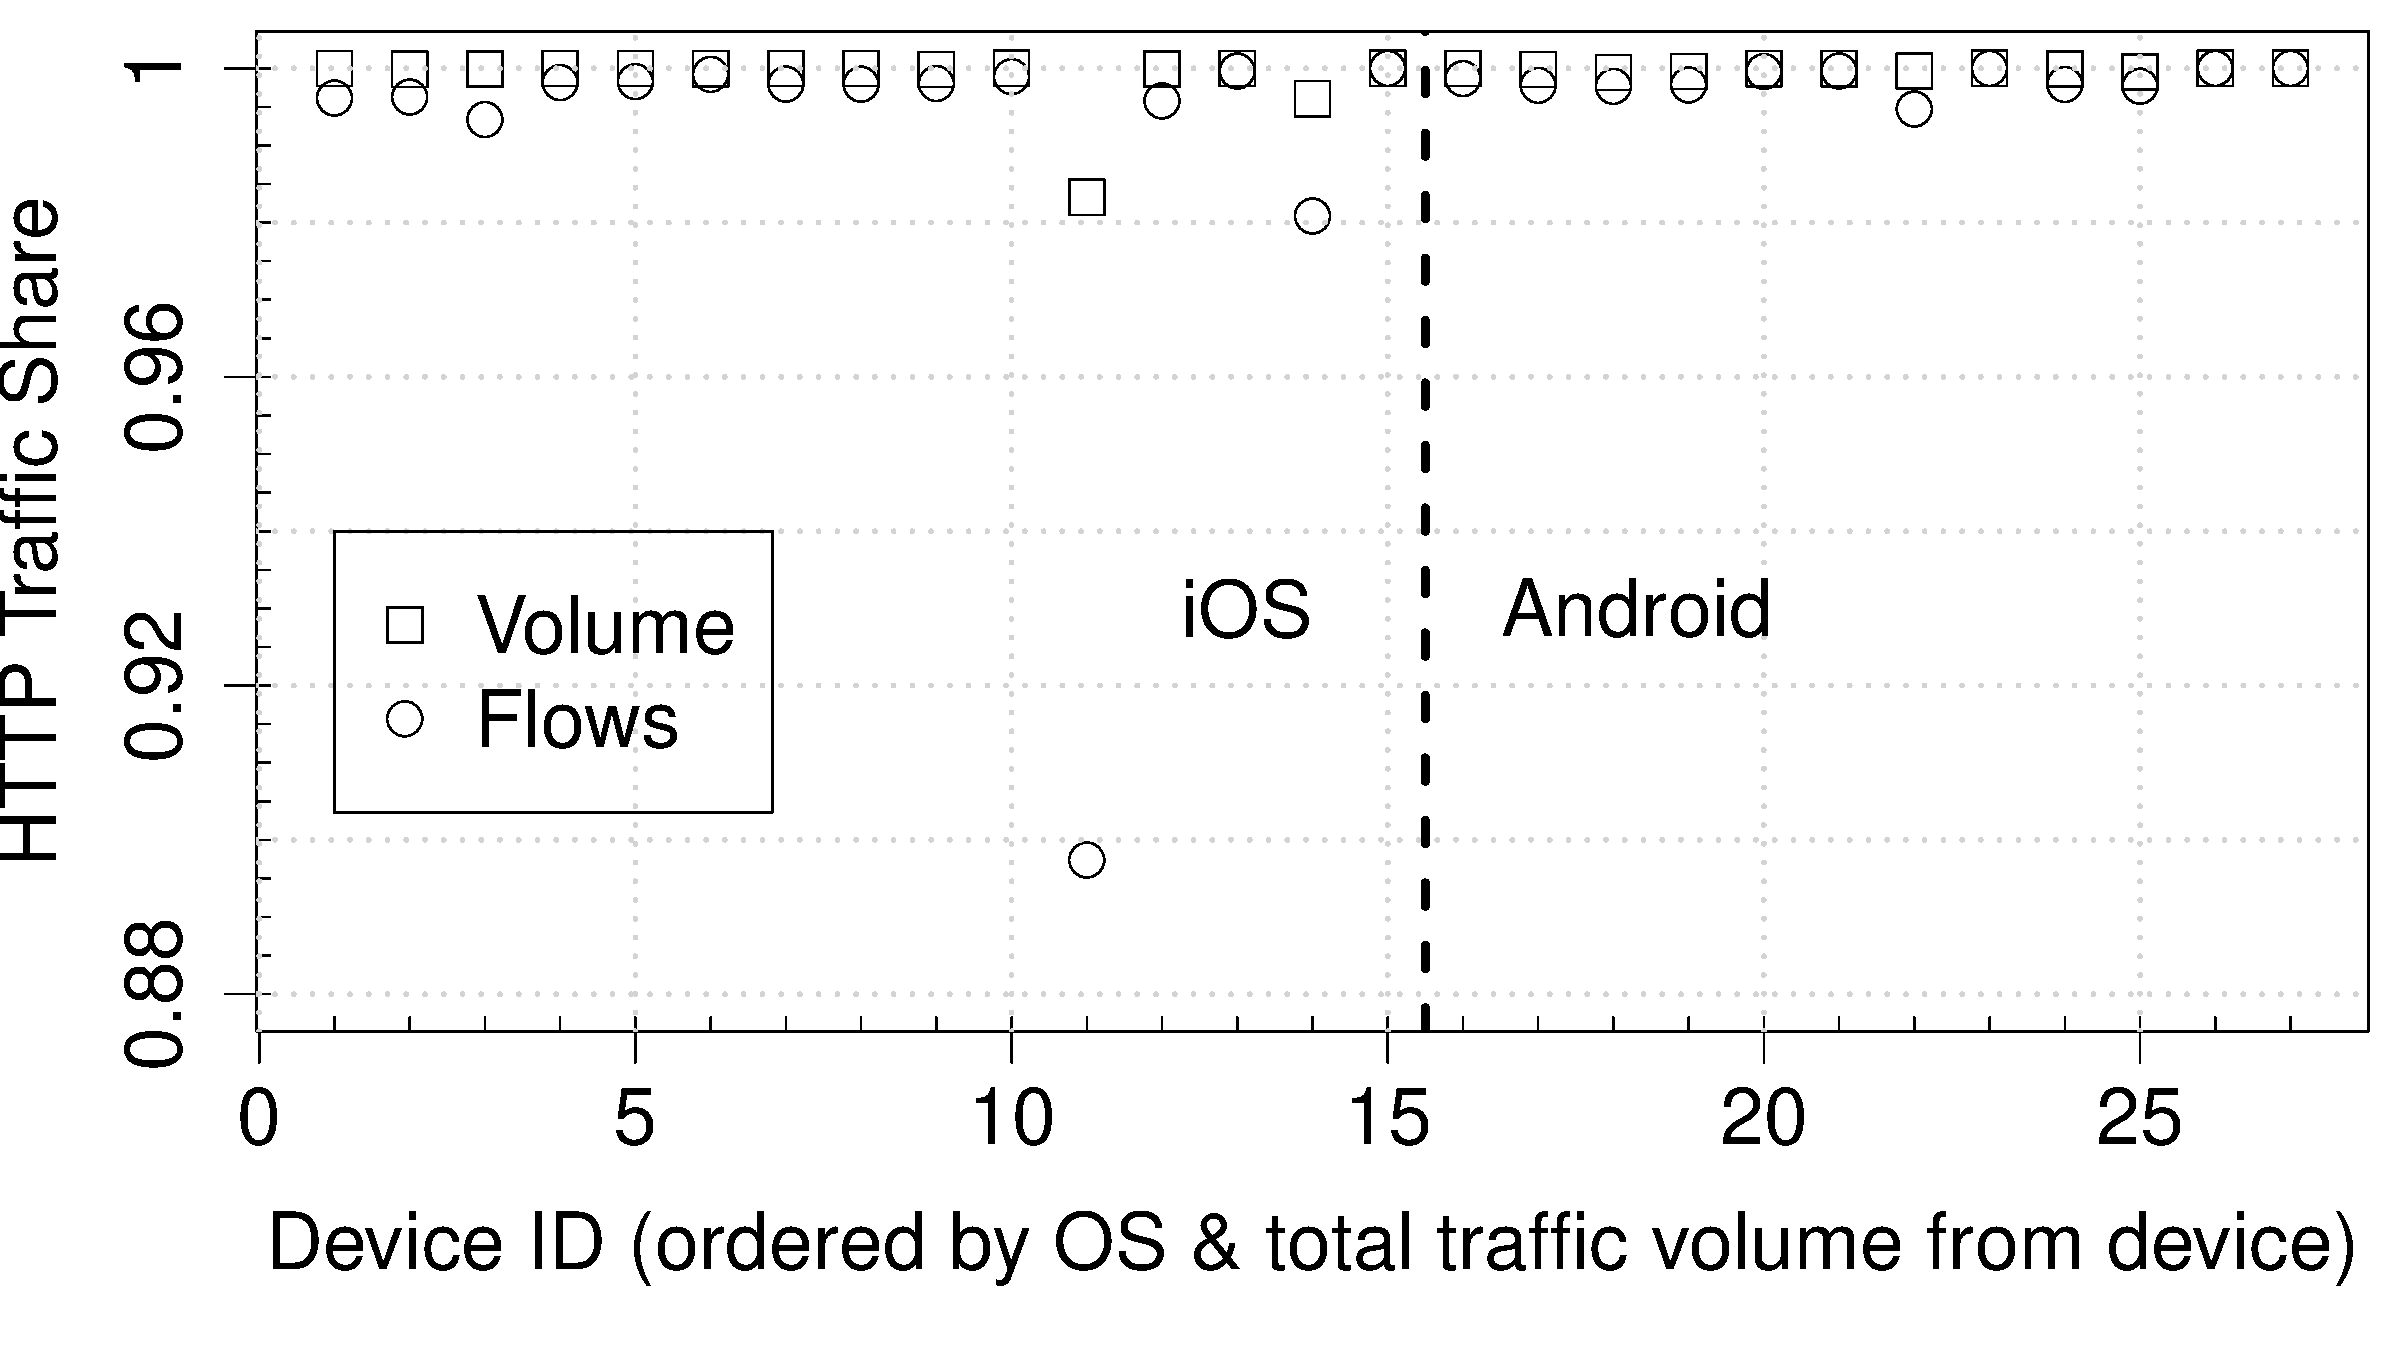
\includegraphics[width=\columnwidth]{plots/appusage_someuseragent_traffic.pdf}
\caption{HTTP traffic with a User-Agent.}
\label{fig:http-classification-some-user-agent}
\end{figure}

We observe that more than 98\% of HTTP traffic from the iOS and Android devices have a valid User-Agent string. \tbd{\fref{fig:http-classification-some-user-agent}}).
In the 95.96 GB of data traffic, we observed a total of 1435 unique User-Agent strings.
We extract the application identifiers in the User-Agent strings by using regular expressions that replace the OS, carrier, and other auxillary information such as delimiters with a blank character.
We then cluster these blank separated tokens based on the number of similar tokens.
We further cluster these clustered tokens using the edit distance. 
At the end of this process we were able to identify 361 unique application signatures.
We use the extracted application signature to label the HTTP traffic that flows through \platname.

\begin{figure}
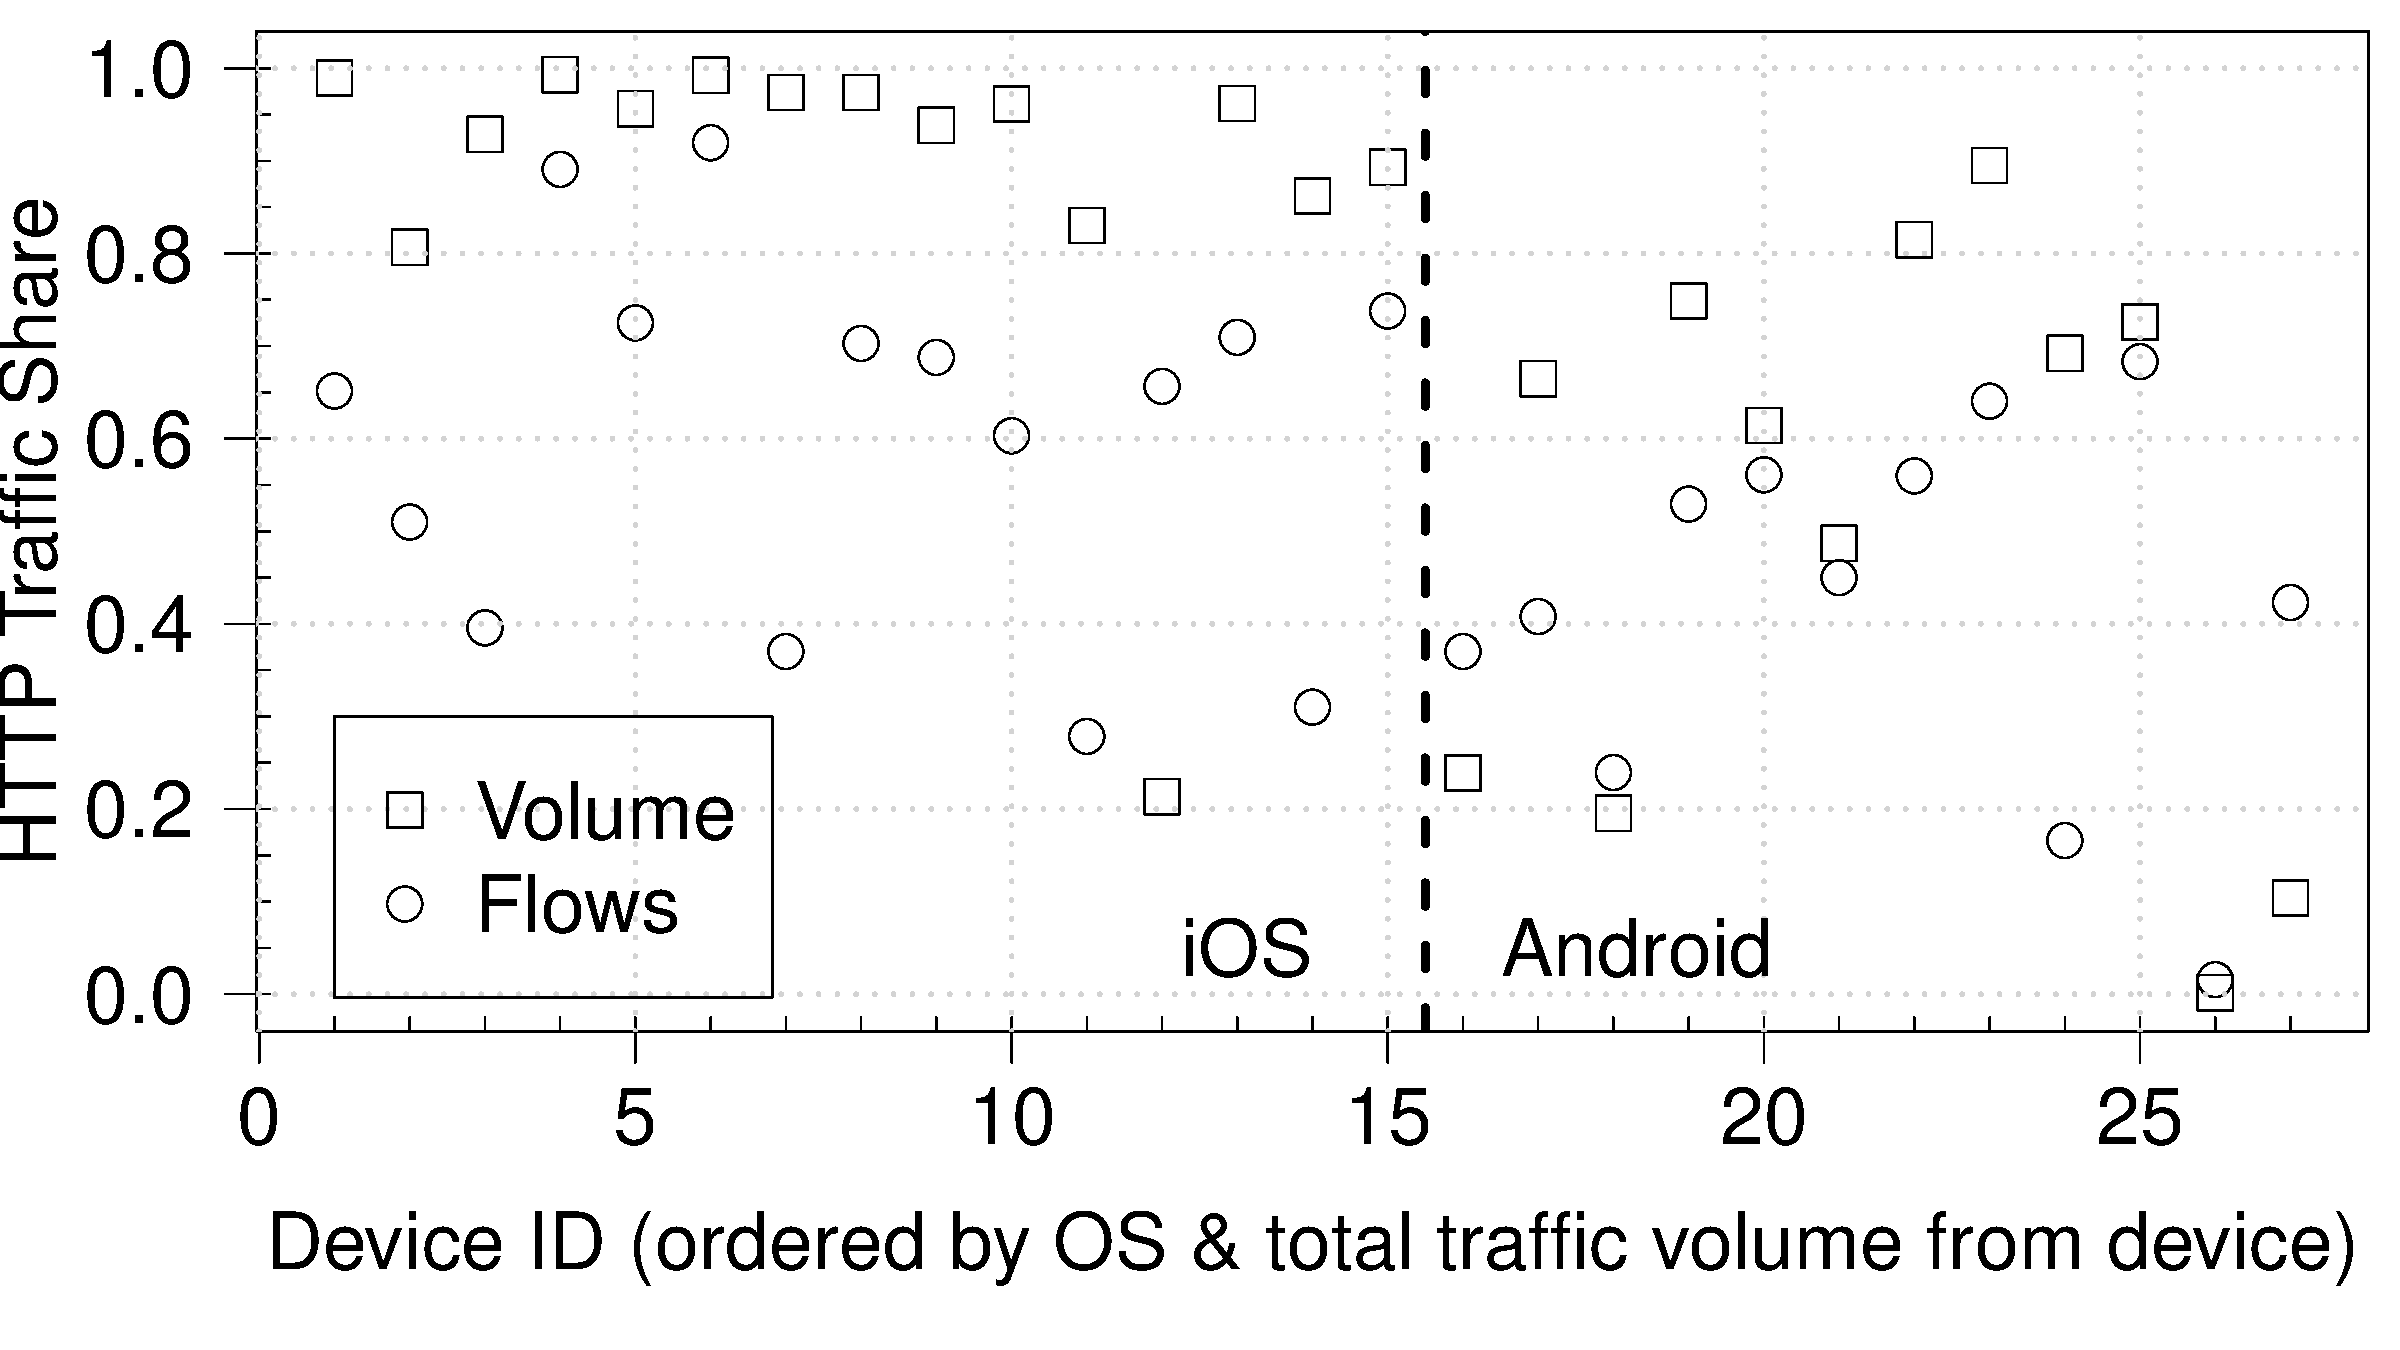
\includegraphics[width=\columnwidth]{plots/appusage_someappsig_traffic.pdf}
\caption{HTTP traffic with a User-Agent with an identifier of an application or OS service.}
\label{fig:http-classification-app-user-agent}
\end{figure}

In \fref{fig:http-classification-app-user-agent} we plot the fraction of HTTP traffic for which an application signature for found; the devices are ordered according to the operating system, and for each operating system we further order the devices according to the total traffic from the device that flowed through \platname. 
We observe that a significantly larger fraction of traffic from iOS device can be mapped to an application in comparison to the traffic from Android devices. 
For example, while more than 80\% of HTTP traffic from iOS device was labeled to an application, we were able to classify only 23.9\% of 9.6~GB of HTTP traffic from device 16 and 19.5\% of the 2.6~GB of HTTP traffic from device 18.
This difference is because of the techniques used by Android and iOS application to download audio and video content. 

\begin{table}
\begin{tabular}{|l|l|}
\hline
User-Agent Prefix& OS \tabularnewline
\hline
AppleCoreMedia/1.0 & iOS \tabularnewline
stagefright/1.2 & Android \tabularnewline
Dalvik/1.6 & Android \tabularnewline
Linux; Android & Android \tabularnewline
com.google.android.youtube & Android \tabularnewline
\hline
\end{tabular}
\caption{Prefix of User-Agent string while streaming youtube videos. \emph{While iOS devices use AppleCoreMedia for more than 95\% of YouTube traffic, Android devices use a variety of User-Agent strings depending on the Android version, YouTube application version, and the version of various applications from which YouTube videos are viewed.}}
\label{tab:top-user-agents}
\end{table}

The iOS devices use the AppleCoreMedia service to download audio and video content. 
For example, we observed that AppleCoreMedia was mentioned in the User-Agent string for 98.45\% of the content downloaded from the YouTube servers. 
We classify YouTube servers based on the host name specified the HTTP GET requests. 
We observed that AppleCoreMedia was the primary application that fetched content from other media sites such as Netflix and iTunes.
Like iOS devices have AppleCoreMedia, Android provides Stagefright\cite{stagefright} as media library.
However, only 41.91\% of YouTube content in our dataset was fetched using Stagefright in the User-Agent field. 
In contrast, 56.52\% of YouTube content was downloaded by Android devices without any application signature in the User-Agent field.  

\begin{figure}
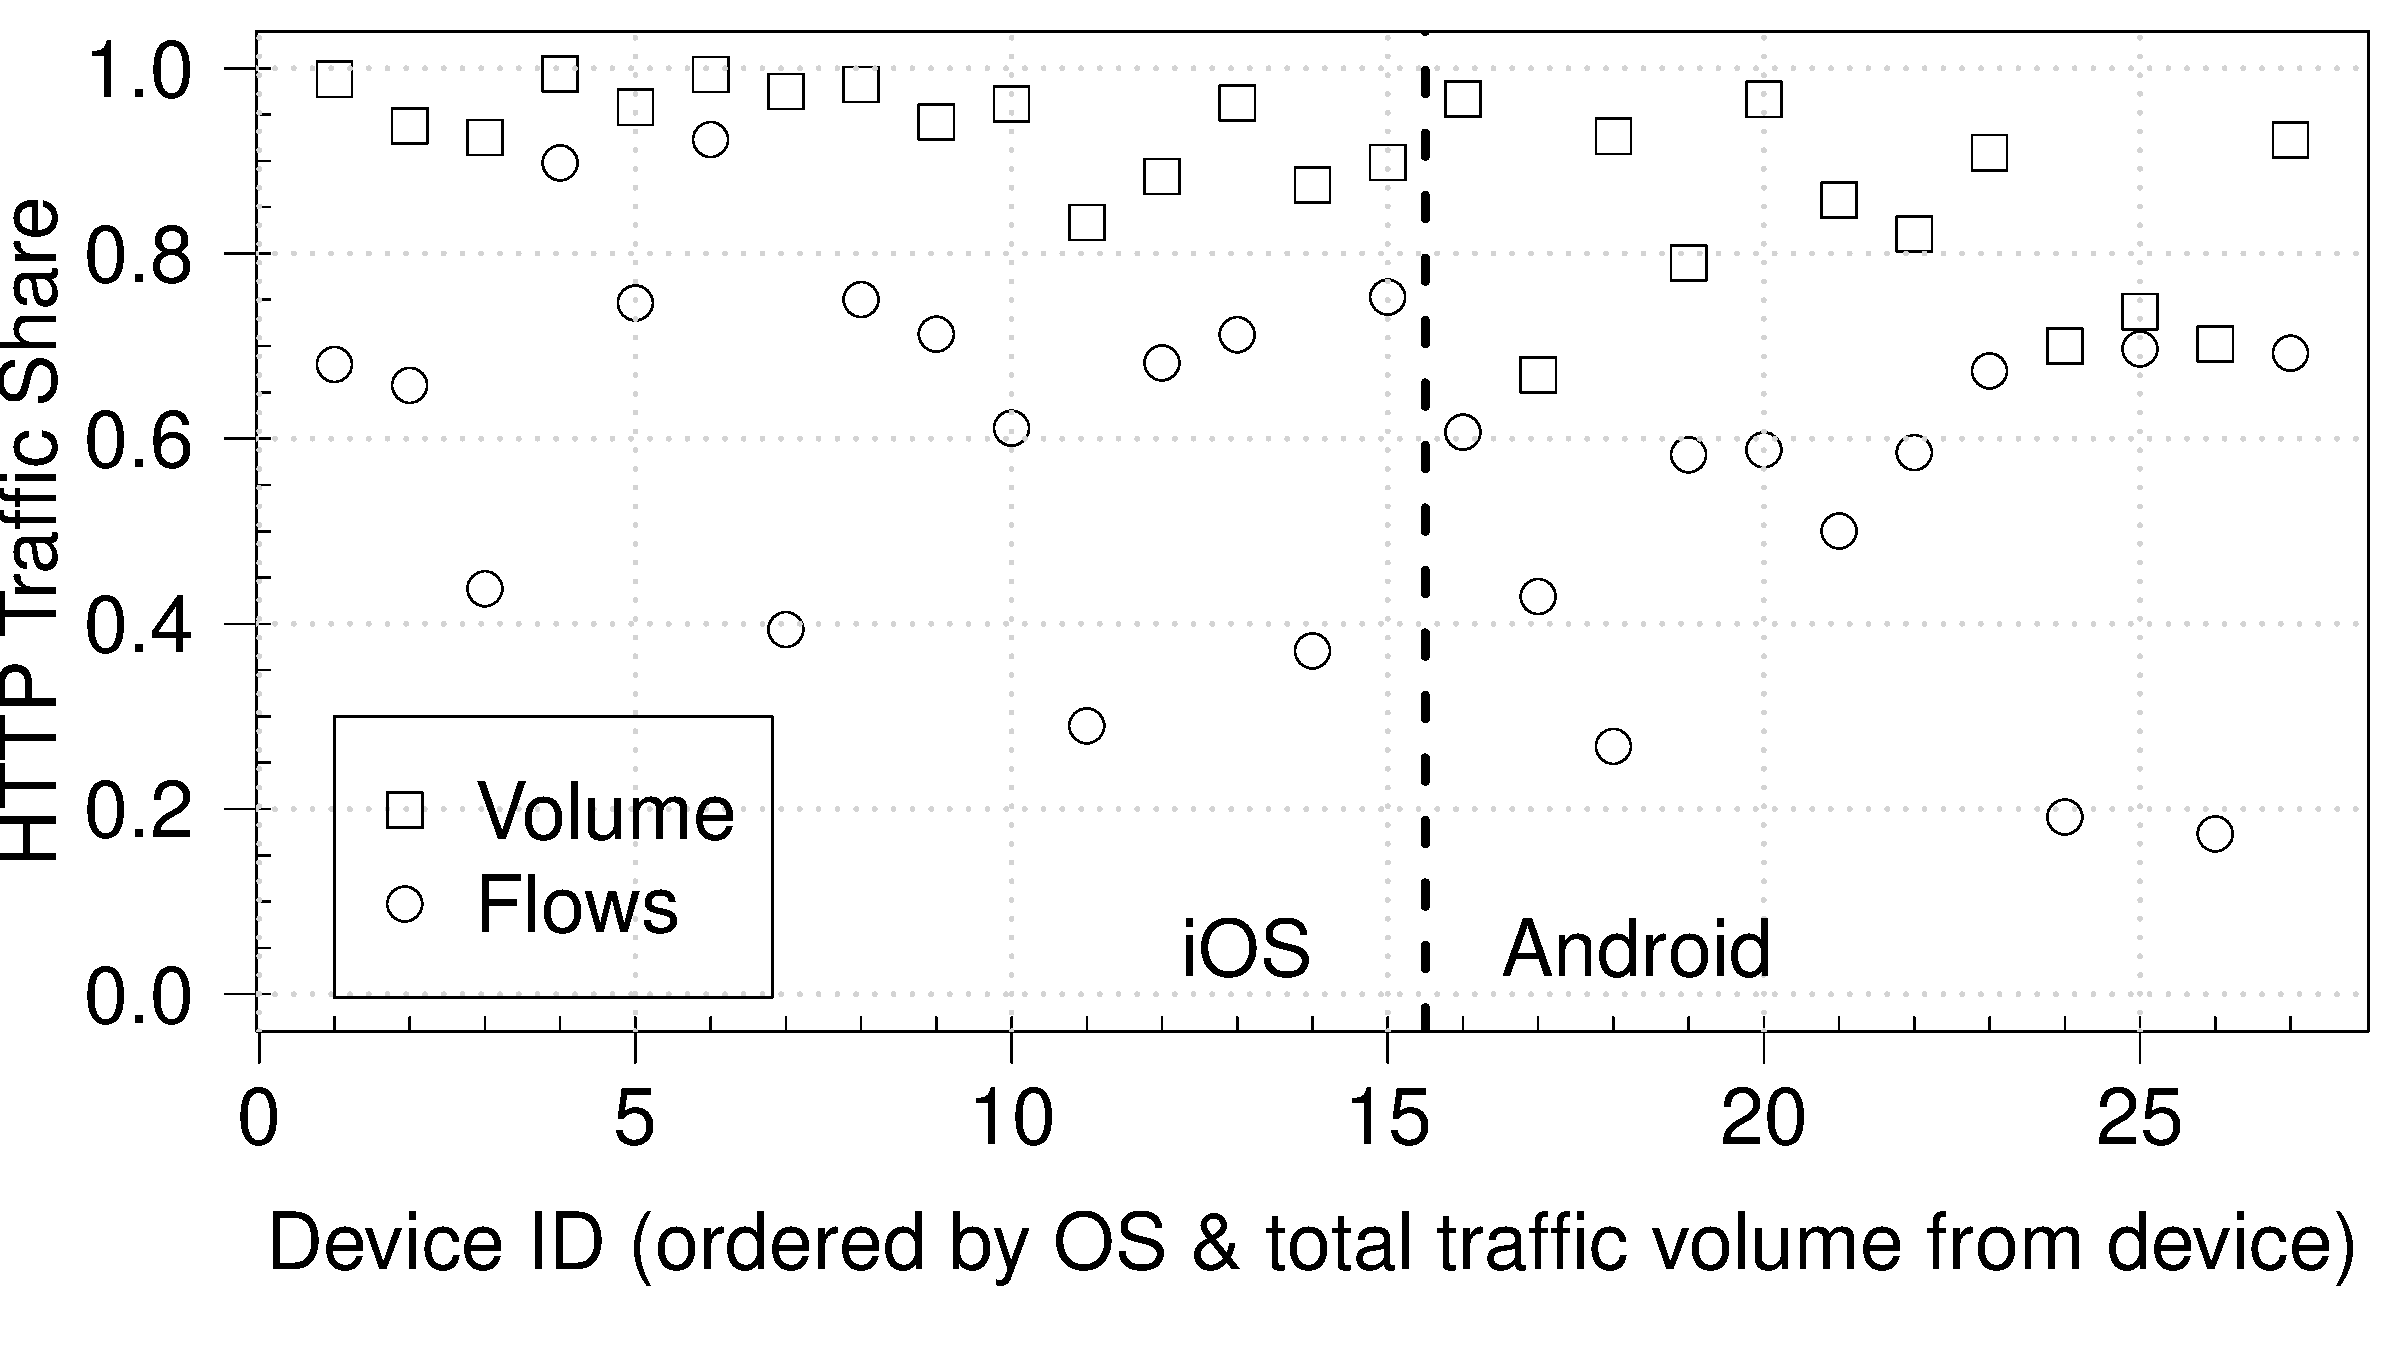
\includegraphics[width=\columnwidth]{plots/appusage_someappservicesig_traffic.pdf}
\caption{HTTP traffic classification using User-Agent or name of media service.}
\label{fig:http-classification-app-service}
\end{figure}
To further classify the media content, we use the \emph{HOST} field in the HTTP GET requests.
We assign flows a label based on the host names of popular media sites. 
In \fref{fig:http-classification-app-service} we plot the fraction of traffic that we could classify by using the User-Agent along with the host names. 
We observe that despite this technique the traffic share of classified traffic for Android devices still lags behind that of iOS devices. 

What we show
Difference in media content download in iOS and Android
The fields in the HTTP requests that can be used to classify HTTP content and identify traffic sources. 
The difference in the use of UserAgents in Android and iOS. 

\subsection{Classification of SSL Traffic}

Field observed in traffic:
server name and the 
Use of subject field in the certificates. 
Issues with generic certificates CN=*.google.com.
Workaround:
Use of DNS

\cite{chen:wifi}


\begin{figure}
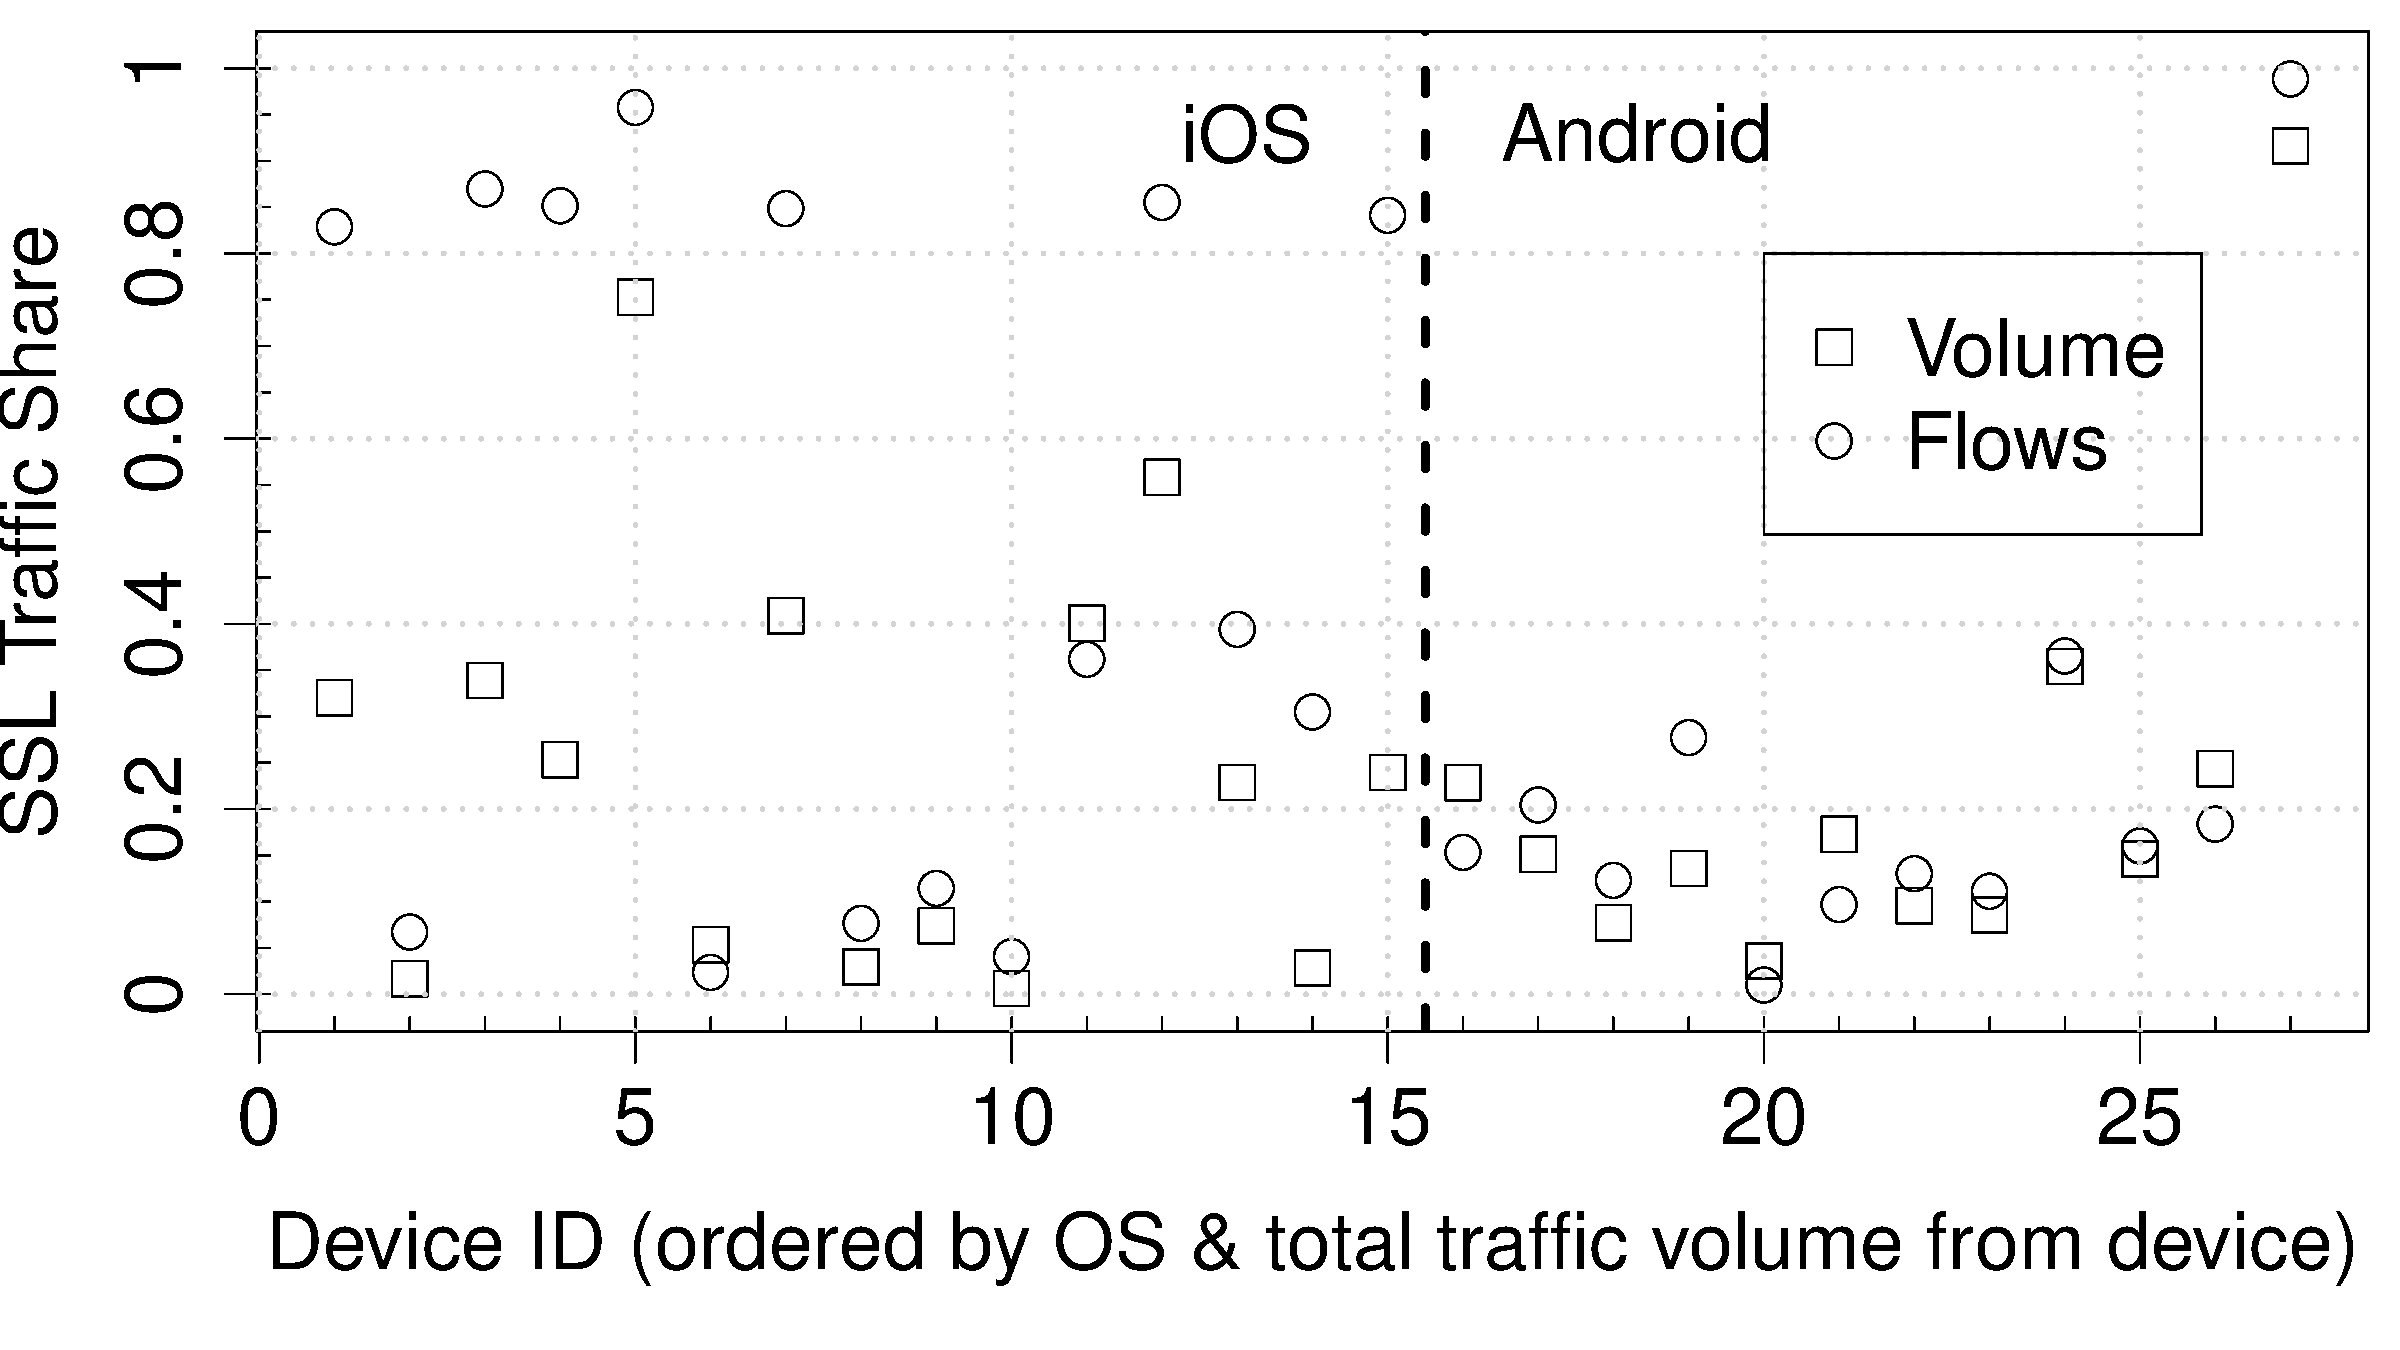
\includegraphics[width=\columnwidth]{plots/sslanalysis_someservername_traffic.pdf}
\caption{HTTP traffic classification using User-Agent or name of media service.}
\label{fig:http-classification-app-service}
\end{figure}


\begin{figure}
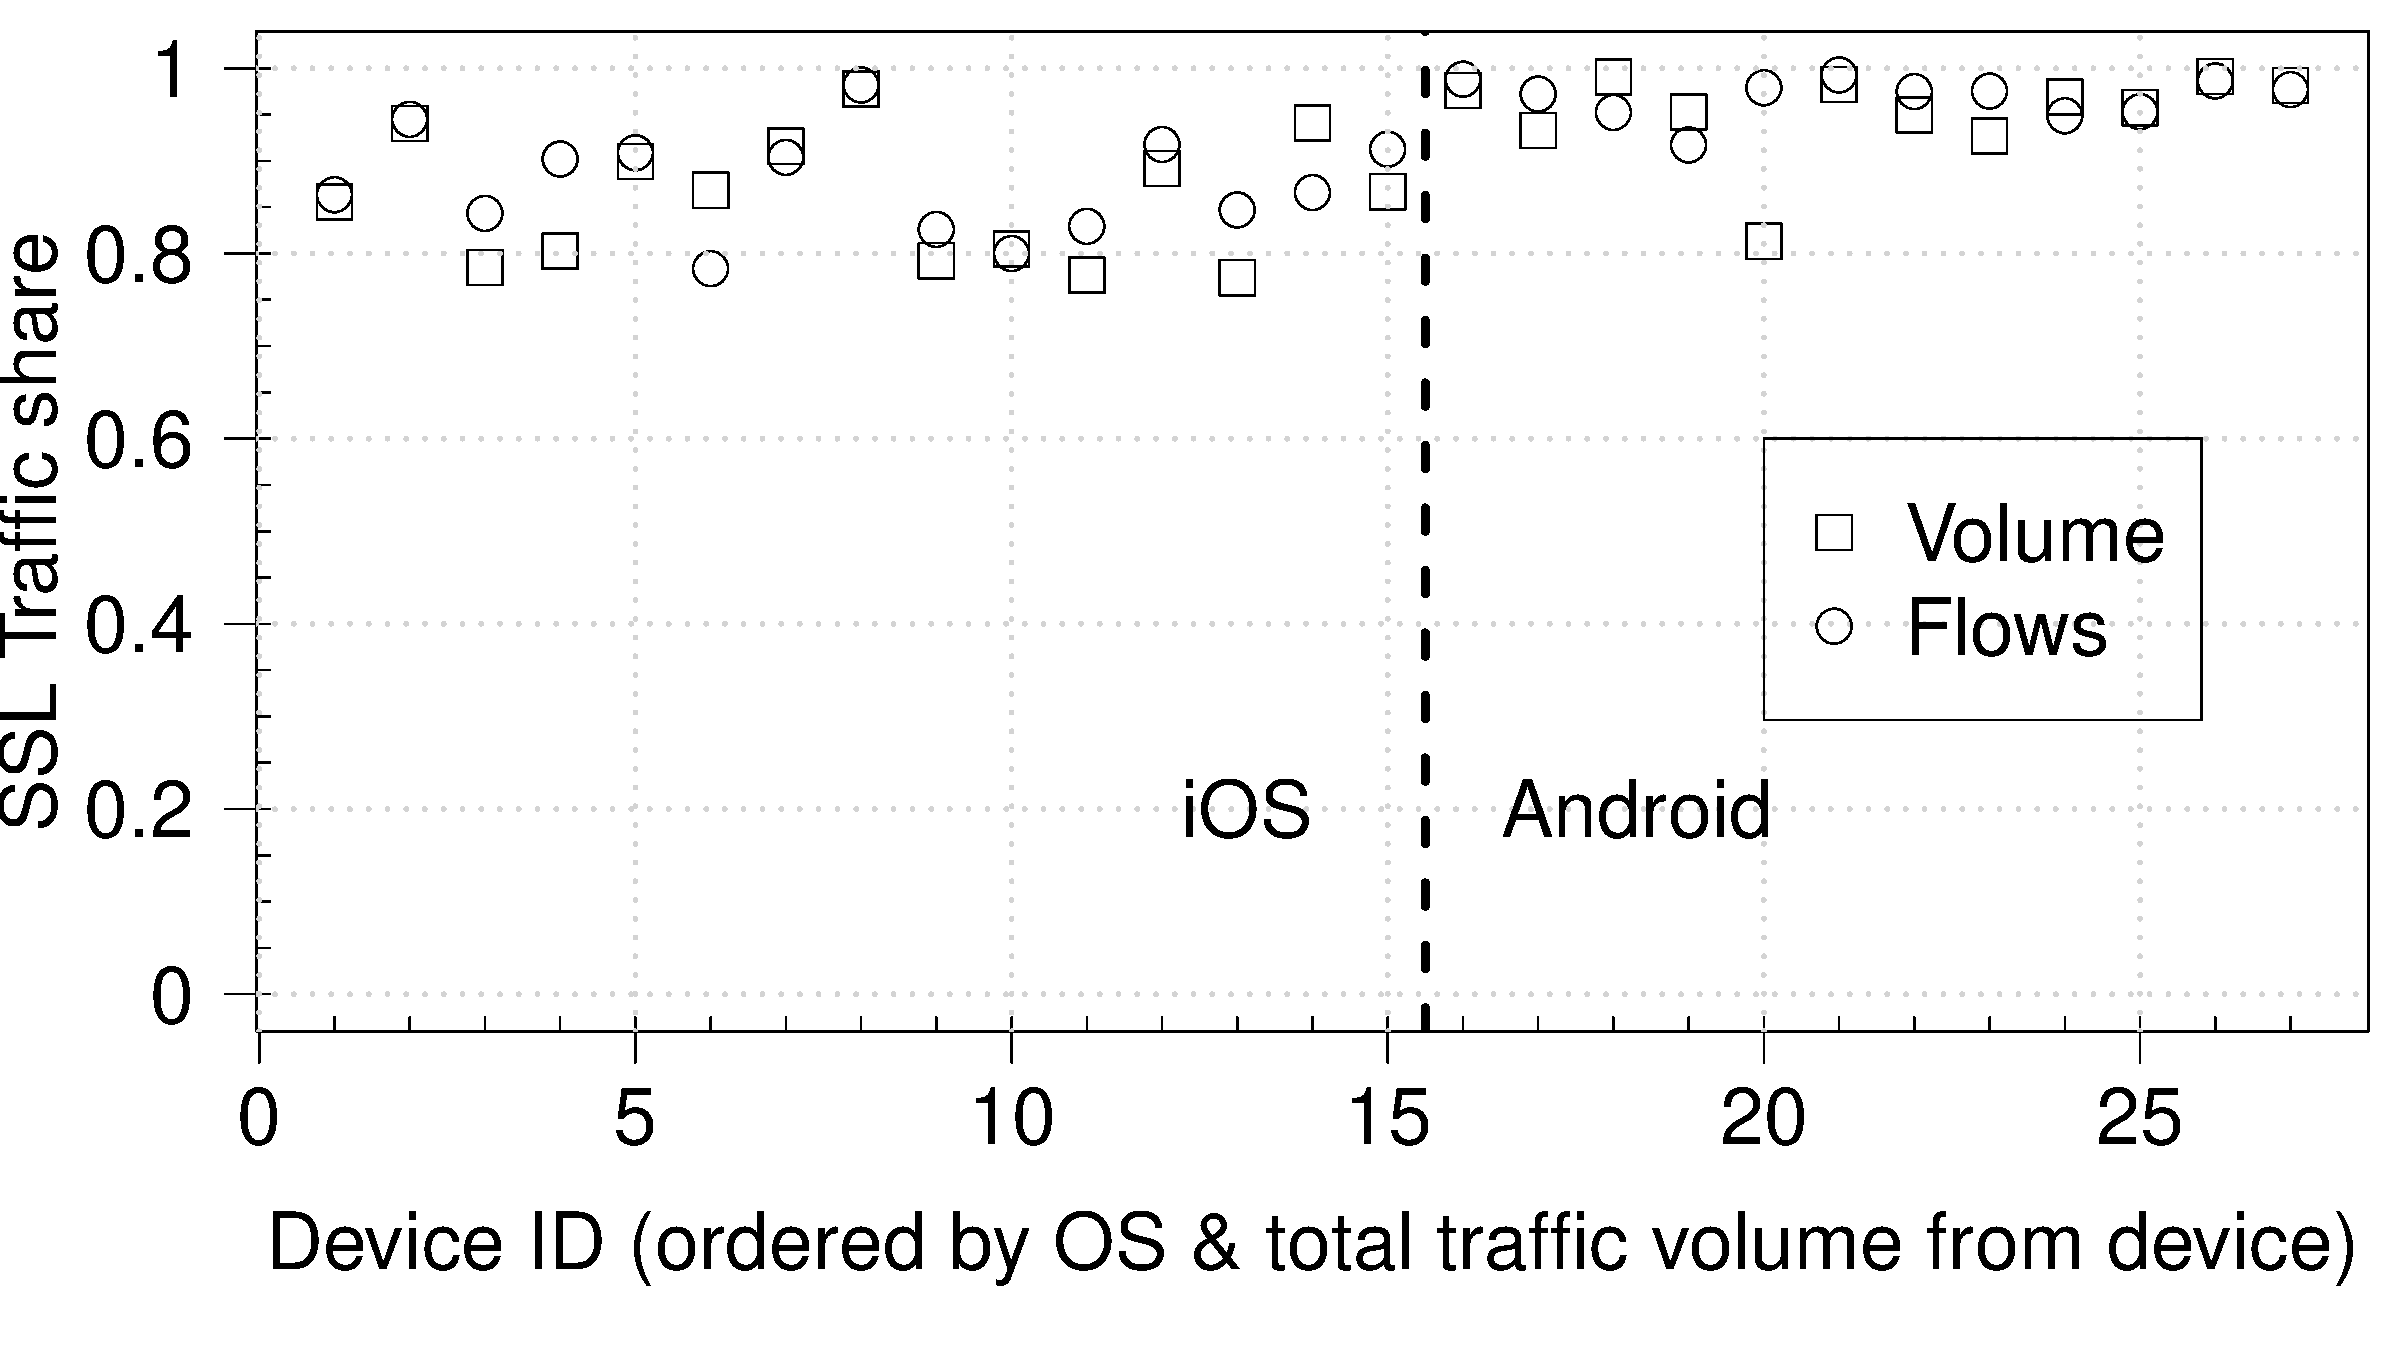
\includegraphics[width=\columnwidth]{plots/sslanalysis_samedns_traffic.pdf}
\caption{HTTP traffic classification using User-Agent or name of media service.}
\label{fig:http-classification-app-service}
\end{figure}


\begin{figure}
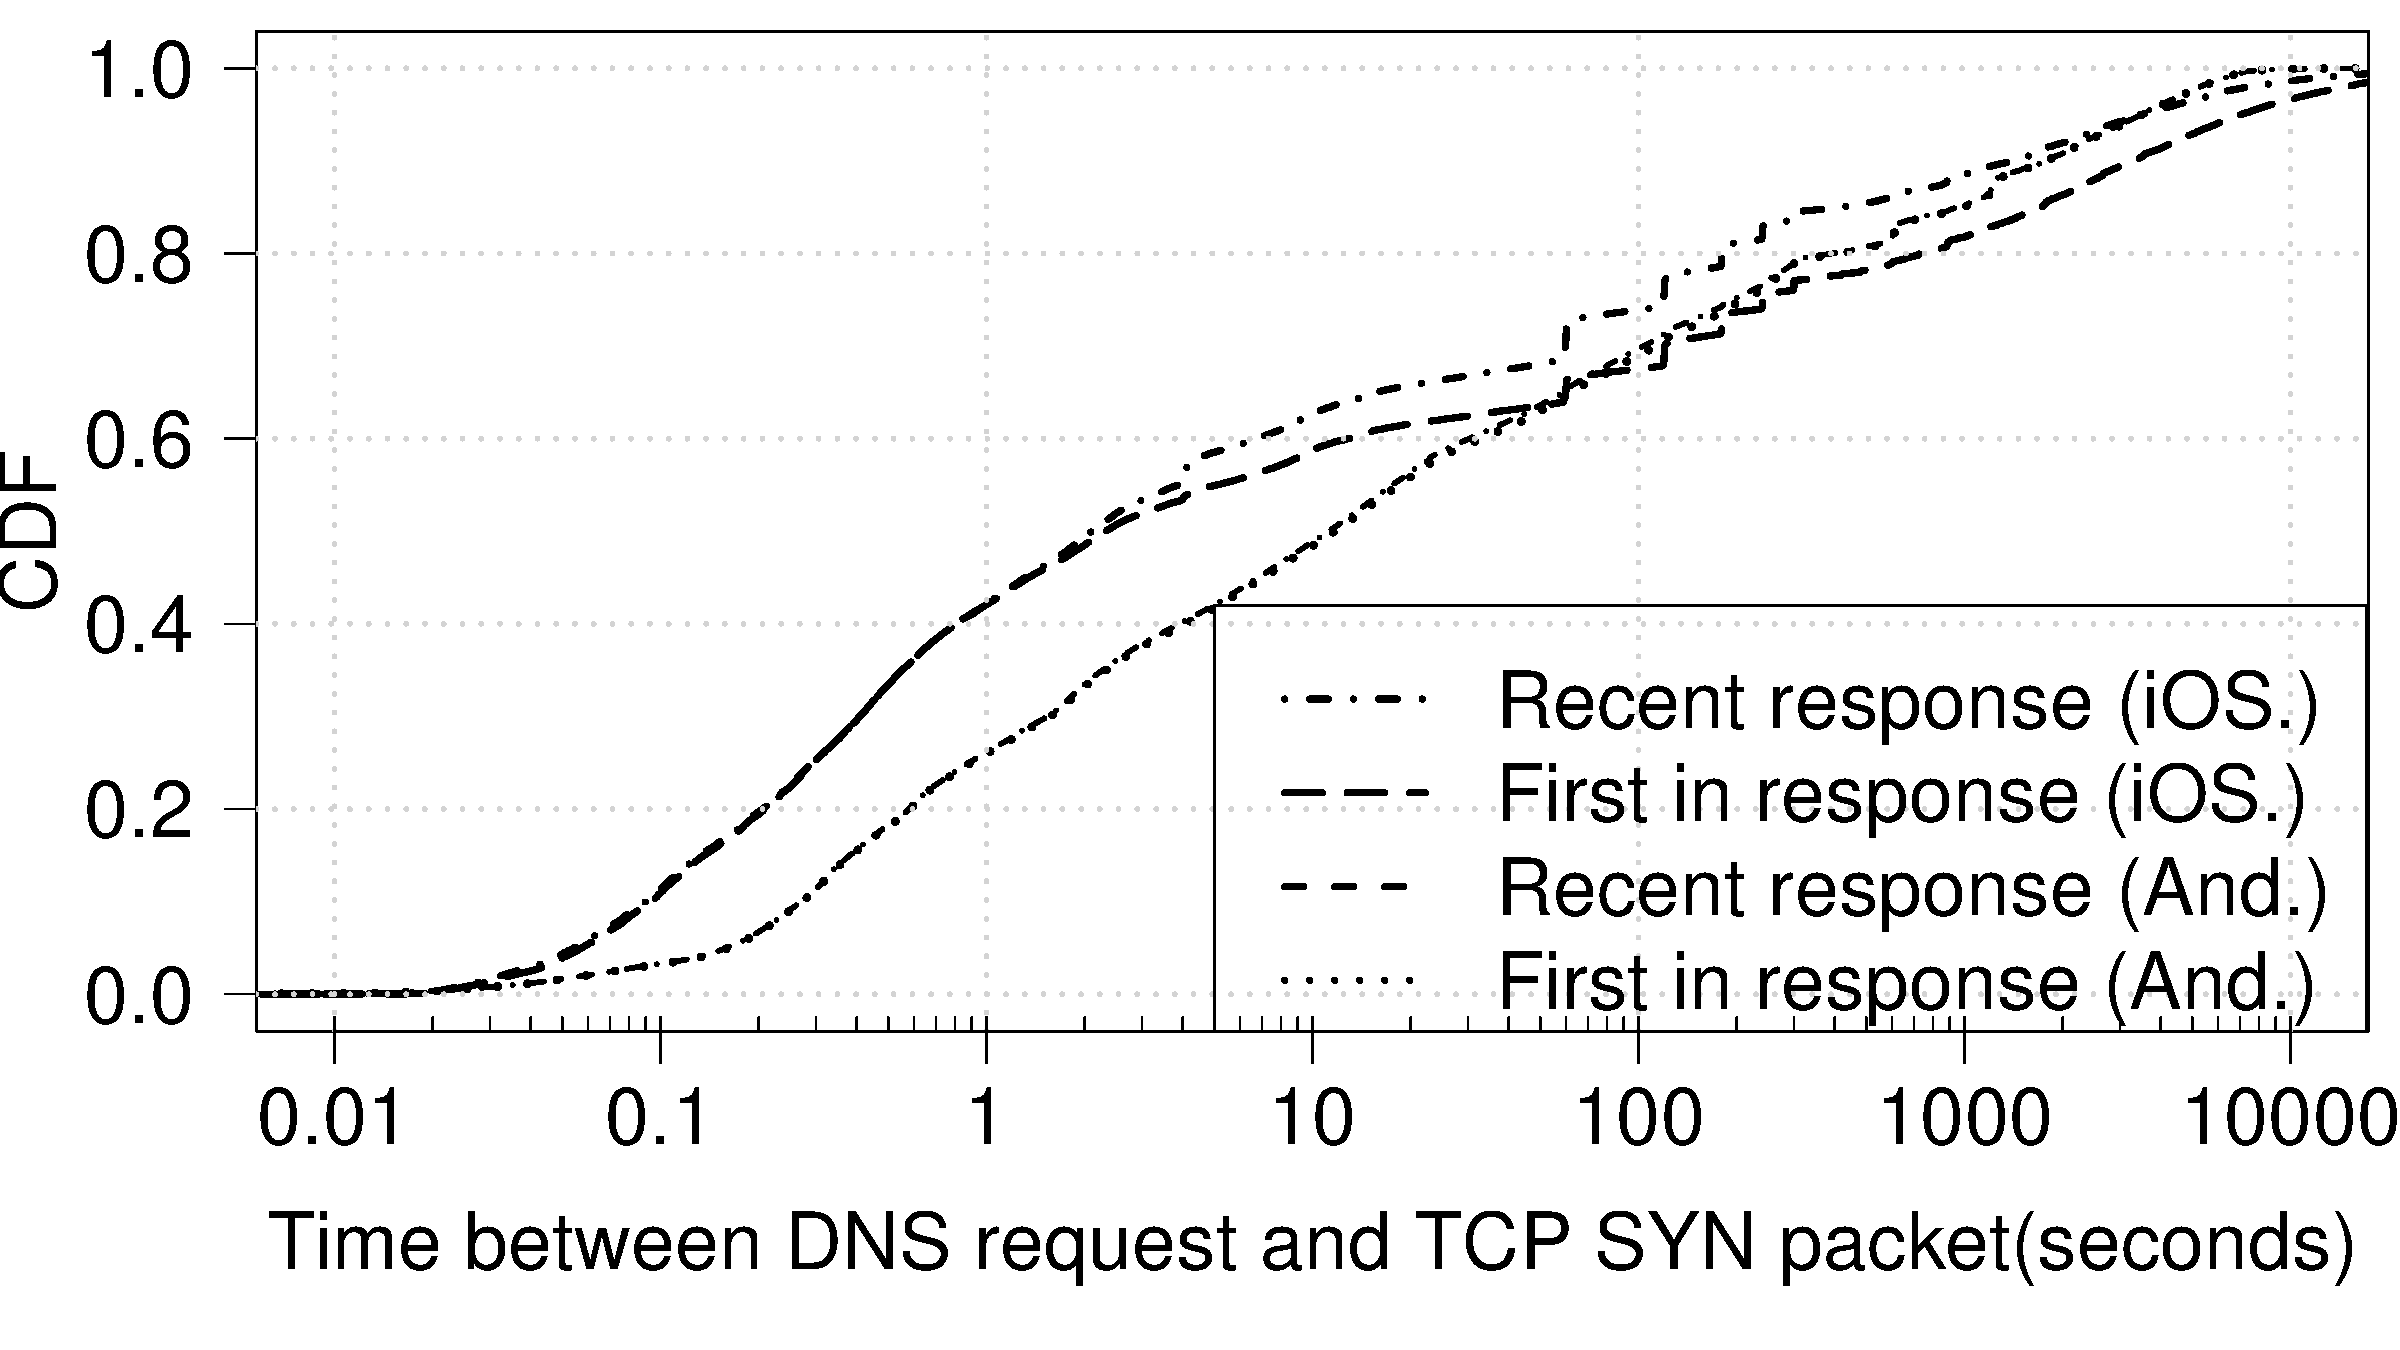
\includegraphics[width=\columnwidth]{plots/sslanalysis_dns_timediff_distrib.pdf}
\caption{HTTP traffic classification using User-Agent or name of media service.}
\label{fig:http-classification-app-service}
\end{figure}



\subsection{Misc}

\begin{table}
\begin{tabular}{|l|l|l|l|}
\hline
\multirow{2}{*}{\bf Hostname} & \multicolumn{2}{|c|}{\bf Number of devices}\tabularnewline
\cline{2-3}
    & {\bf iOS} & {\bf Android} \tabularnewline
\hline
www.facebook.com & 11 & 8 \tabularnewline
b.scorecardresearch.com	& 10 &	5 \tabularnewline
p.twitter.com	& 7 & 1 \tabularnewline
www.google-analytics.com &  6 & 2 \tabularnewline
bcp.crwdcntrl.net & 4 &	3 \tabularnewline
\hline
\end{tabular}
\caption{The top 5 hosts accessed from Android and iOS devices with an empty user agent field}
\label{tab:top-hosts-empty-agent}
\end{table}



%%% Local Variables: 
%%% mode: latex
%%% TeX-master: "../main"
%%% End: 


